\subsection{MEX 1-2: Drying and wetting paths of the Opalinus Claystone}

Participating institutions of MEX 1-2 (see section \ref{sec:mex06}): CAU, UFZ

\begin{table}[ht!]
\caption{MEX 1-2: Data overview}
\label{tab:dms-mex12-overview}
\small
\begin{tabular}{l|l|l|l|L{4.7cm}|l}
\hline
\rowcolor{cyan}
Type & Spec. & Owner & Access     & Comment                       & Stat \\ 
\hline
EXP  &   DRY    & CAU   & Open       & Output files are uploaded          & \cellcolor{green} \\
\hline \hline
MOD  & LEM   & CAU   & Open       & Executable MATLAB P-file               & \cellcolor{yellow} \\
     &       &       & Open       & Input files will be uploaded  & \cellcolor{yellow} \\
\hline
MOD  & FEM   & UFZ   & Open       & Branch to be merged into OGS  & \cellcolor{yellow} \\
     & VPF   &       & Open       & Input files available         & \cellcolor{yellow} \\
%
\hline
\end{tabular}
\end{table}
\normalsize

\subsubsection*{CAU Kiel}

The experimental results of the drying and wetting paths of the sandy Opalinus claystone are uploaded to the IfG (Kiel) NextCloud server. The data is accessible through the following link:\\
\url{https://nextcloud.ifg.uni-kiel.de/index.php/s/q6g25nWyWJKqzNB}

The experimental data (*.xlsx) of drying and wetting paths are uploaded to the server. The data includes the reading number, time (day), stain values in perpendicular and parallel orientations, weight of the sample and measured water content values. Fig. \ref{fig:Amir_ME6_Strain_Data} shows the change of the strains under the applied suction values.

\begin{figure}[!ht]
\centering
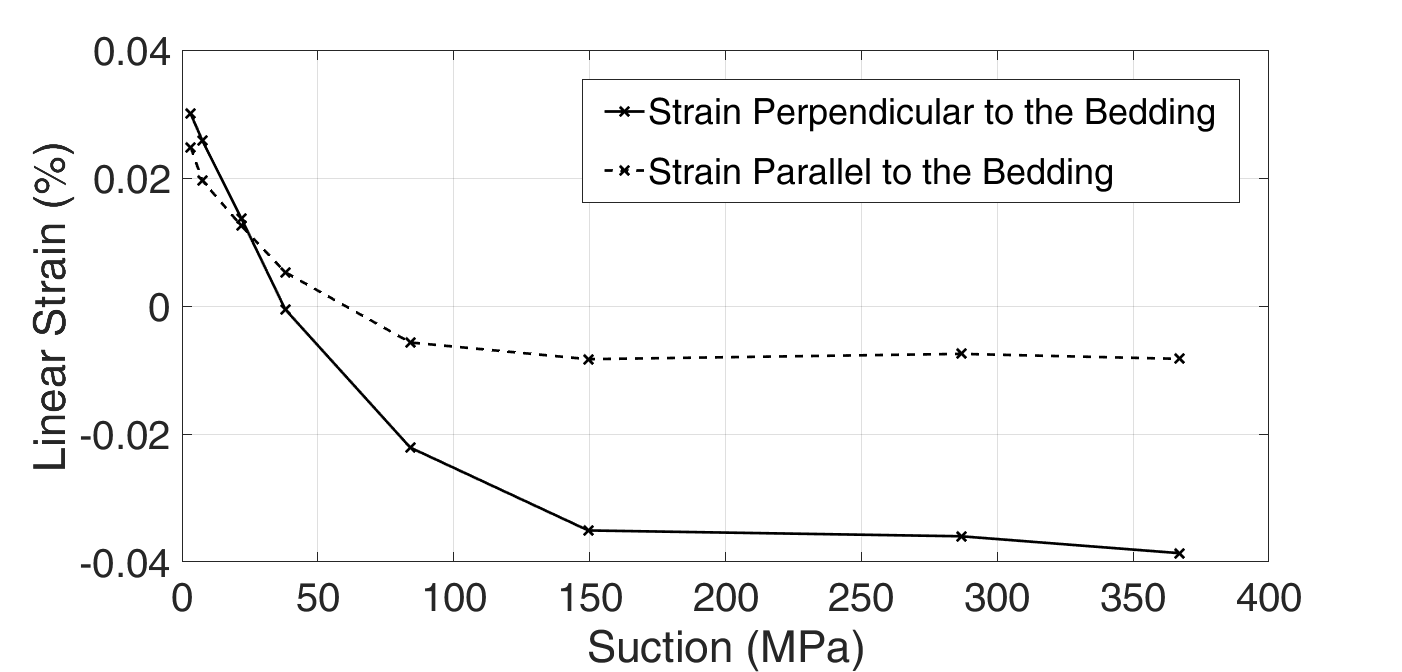
\includegraphics[width=0.75\textwidth]{figures/Amir_ME6_Strain_Data.png}
\caption{The suction vs. linear strains}
\label{fig:Amir_ME6_Strain_Data}
\end{figure}

The required LEM code and the input variables for simulating the drying and wetting paths of the sandy Opalinus claystone are uploaded to the IfG (Kiel) NextCloud server. The data is accessible through the following link:\\
\url{https://nextcloud.ifg.uni-kiel.de/index.php/s/fDNoPoXpXMqeAsK}

The uploaded protected MATLAB file in a *.p format requires a MATLAB version with a built-in Voronoi Tessellation and Delaunay Triangulation functions. Fig. \ref{fig:Amir_ME6_Lattice_Drying_Data} shows the change of hydraulic conductivity with applied linear strains as described in section \ref {sec:mex06}. 

\begin{figure}[!ht]
\centering
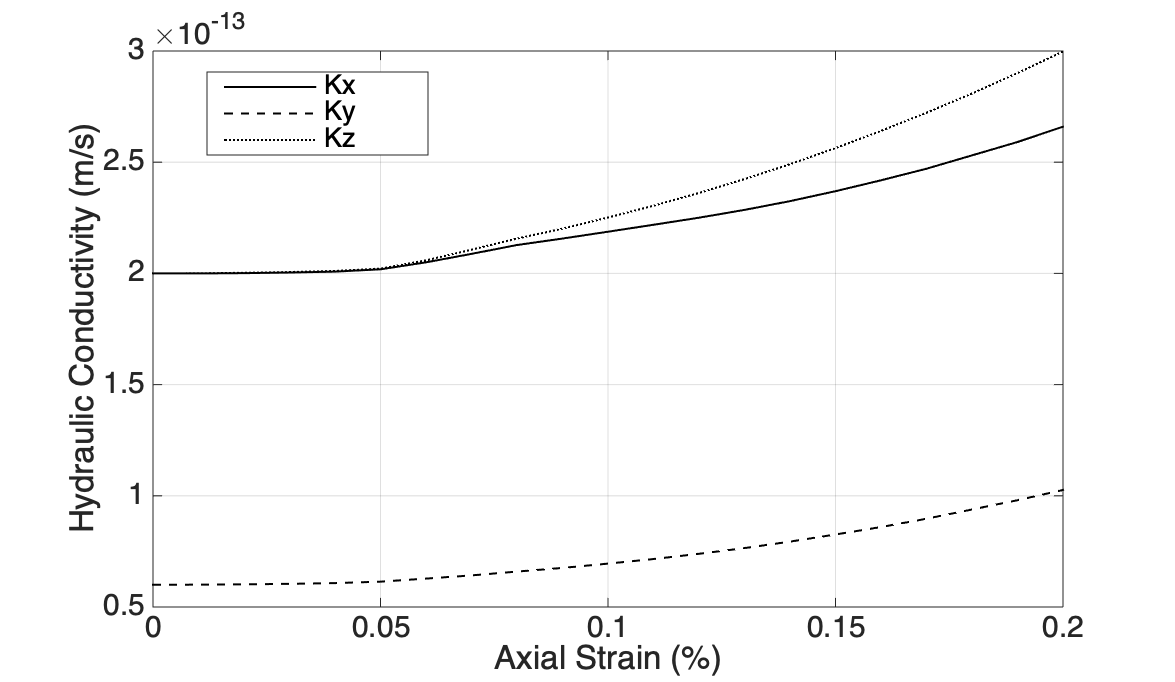
\includegraphics[width=0.6\textwidth]{figures/Amir_ME6_Lattice_Drying_Data.png}
\caption{The change of hydraulic conductivity with applied linear strains, Opalinus claystone}
\label{fig:Amir_ME6_Lattice_Drying_Data}
\end{figure}

%---------------------------------------------------------
\subsubsection*{Meta Data Overview (according to Dublin Core)}
%---------------------------------------------------------

\begin{table}[!ht]
\caption{MEX 1-2 (CAU)}
\label{tab:dms-mex1-2}
\small
\begin{tabular}{R{3.5cm}|L{7.5cm}}
\hline
%
Data label & GeomInt, MEX 1-2, CAU, drying and wetting paths, Opalinus clay \\
URL (Experiments) & \url{https://nextcloud.ifg.uni-kiel.de/index.php/s/q6g25nWyWJKqzNB} \\
URL (Numerics) & \url{https://nextcloud.ifg.uni-kiel.de/index.php/s/fDNoPoXpXMqeAsK} \\
Subject  &  Drying and Wetting Paths (Opalinus claystone)\\
Type of data  & Experimental data, executable MATLAB P-file, input parameters\\
Data quality  &  Quality assured data \\
Status of data  &  Unprocessed data\\
Data format  & txt, xlsx, MATLAB executable P-file\\
Creators  &  Kiel University, Institute of Geomechanics and Geotechnics, Ludewig-Meyn-Stra\ss e 10, 24118, Kiel\\
Source/Origin & In-house code \\
Publisher  &  Kiel University, Institute of Geomechanics and Geotechnics, Ludewig-Meyn-Stra\ss e 10, 24118, Kiel \\
Rights holders &  Kiel University, Institute of Geomechanics and Geotechnics, Ludewig-Meyn-Stra\ss e 10, 24118, Kiel \\
Contributors &   Kiel University, Institute of Geomechanics and Geotechnics: Amir Shoarian Sattari, Frank Wuttke\\
Time/period of creation &  2018-2020\\
Language of the content &  English\\
Update policy &  Stored data is final\\
Access permissions & Full access\\
%
\hline
\end{tabular}
\end{table}